\chapter{Analisis}
\label{chap:analisis}

Pada bab ini dijelaskan mengenai ....

\section{Leksikon}
\label{sec:leksikon}
Leksikon, seperti dijelaskan pada subbab \ref{sec:morfemDasarDLL}, dapat dipadankan dengan istilah \textit{kosakata} atau \textit{perbendaharaan kata}. Leksikon dibutuhkan pada proses \textit{morphological parsing} untuk mengetahui apakah sebuah kata yang sedang diproses adalah sebuah bentuk dasar yang valid atau tidak dalam bahasa Indonesia. Leksikon menyimpan kumpulan bentuk dasar dan turunannya untuk nantinya diakses ketika proses \textit{morphological parsing} dilakukan.

Leksikon dalam proses \textit{morphological parsing} harus bisa diakses dengan cepat dan efektif. Hal ini dikarenakan leksikon akan diakses sangat sering dalam proses ini. Leksikon akan diakses sekitar 3-5 kali untuk setiap kata yang sedang diproses. Oleh karena itu, leksikon perlu disimpan pada struktur data yang memungkinkan waktu akses yang cepat supaya keseluruhan proses dapat dijalankan dalam waktu yang masuk akal. 

Struktur data yang saat ini terkenal paling cepat untuk diakses adalah struktur data \textit{trie}. Trie adalah struktur data berbentuk pohon yang menyimpan himpunan string yang jika ditelusuri setiap node mulai dari akar hingga daun akan membentuk suatu string yang merupakan kunci yang kita cari. Setiap string yang dihasilkan dari node awal yang sama akan mempunyai awalan (prefiks) yang sama, karena itulah trie disebut juga pohon prefiks.

\begin{figure}[H]
\centering
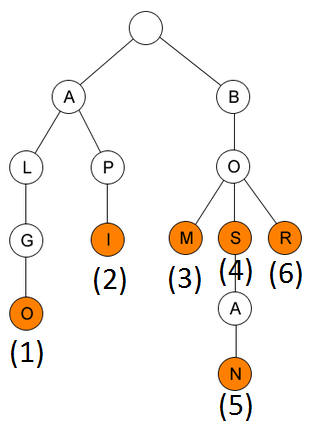
\includegraphics[scale=0.75]{Gambar/gambar-trie}
\caption[Struktur data trie]{Struktur data trie} 
\label{bagan-trie}
\end{figure}

Struktur data trie yang digambarkan pada bagan \ref{bagan-trie} menyimpan enam string kunci dari dua buah awalan, yaitu string "A" dan "B". Jika kita telusuri dari node akar "A" sampai node daun "O", kita akan mendapat string "ALGO" yang ditandai dengan nomor (1). String lain yang disimpan pada contoh tersebut adalah string "API" pada nomor (2), string "BOM" pada nomor (3), string "BOS" pada nomor (4), string "BOSAN" pada nomor (5), dan string "BOR" pada nomor (6).

Perlu diperhatikan bahwa sebuah string kunci tidak harus disimpan dengan node terakhir ada pada posisi daun, seperti pada string "BOS" pada nomor 4. Node terakhir pada string tersebut merupakan node internal. Penyimpanan seperti ini bisa dilakukan dengan menandai setiap node yang merupakan akhir dari sebuah string yang membentuk kata.

Kata yang disimpan dalam leksikon terdiri dari dua jenis kata, yaitu kata dasar dan kata turunan. Contoh kata dasar adalah kata 'makan', 'sapu', dan 'kerja' sementara contoh kata turunan adalah kata 'makan-makan', 'menyapu', dan 'kerja bakti'. Kata-kata turunan disimpan sebagai bagian dari kata dasar dan dapat diakses ketika dibutuhkan. Dalam Kamus Besar Bahasa Indonesia Dalam Jaringan (KBBI daring)\footnote{https://kbbi.kemdikbud.go.id/}, kata dasar dan kata turunan disimpan secara terpisah namun keduanya dapat diakses melalui cara yang sama, yaitu dengan menuliskannya pada kolom pencarian. Sementara pada Kamus Besar Bahasa Indonesia Luar Jaringan (KBBI luring)\footnote{http://ebsoft.web.id/kbbi-kamus-besar-bahasa-indonesia-offline-gratis/}, hanya kata dasar saja yang bisa diakses dengan menuliskannya pada kolom pencarian. Pada penelitian kali ini akan digunakan struktur penyimpanan seperti pada KBBI luring.

Struktur penyimpanan seperti pada KBBI luring memungkinkan untuk mengenali perbedaan antara kata dasar dan kata yang telah melalui proses morfologi seperti afiksasi, reduplikasi, dan komposisi. Perangkat lunak yang dirancang pada penelitian ini harus dapat menentukan apakah sebuah kata merupakan kata dasar yang valid dalam bahasa Indonesia.


\section{Proses \textit{Morphological Parsing}}
\label{sec:morphologicalParsing}

Pada subbab \ref{sec:prosesMorfologi} telah dibahas mengenai proses morfologi, yang pada dasarnya adalah proses pembentukan kata melalui beberapa proses, yaitu pembubuhan afiks (afiksasi), pengulangan (reduplikasi), penggabungan (komposisi), pemendekan (akronimisasi), dan pengubahan status (konversi). Proses \textit{morphological parsing} merupakan kebalikan dari proses morfologi. Masukan bagi proses \textit{morphological parsing} adalah kata atau kalimat yang telah melalui proses morfologi dan keluarannya adalah komponen-komponen penyusunnya.

Proses \textit{morphological parsing} untuk setiap kata dalam masukan dapat dituliskan sebagai berikut:
\begin{enumerate}
	\item Periksa leksikon, jika kata tersebut ada dalam leksikon, masukkan sebagai salah satu kemungkinan keluaran
	\item Periksa adanya simbol penghubung (-), yang menandakan hasil proses reduplikasi, lalu lakukan pemisahan kata dan lakukan proses parsing pada kedua kata tersebut
	\item Jika ada kata yang mengikuti, periksa kemungkinan kata yang sedang diproses dan kata yang mengikuti adalah dua kata hasil komposisi, lalu lakukan proses parsing pada kedua kata tersebut
	\item Periksa adanya kemungkinan afiks, baik itu prefiks, sufiks, infiks, maupun konfiks. Pisahkan afiks yang ditemukan dengan komponen kata yang lain dan lakukan pengecekan leksikon pada komponen kata tersebut
	\item Jika sudah dilakukan pemisahan terhadap kemungkinan afiks namun kata yang sedang diproses tidak ditemukan dalam leksikon, kemungkinan kata tersebut bukan kata dalam bahasa Indonesia
\end{enumerate}

Sebagai contoh, jika dilakukan proses \textit{morphological parsing} pada kata 'kemerah-merahan', maka prosesnya adalah sebagai berikut:
\begin{itemize}
	\item Periksa leksikon, kata tersebut tidak ditemukan dalam leksikon
	\item Ditemukan simbol penghubung (-) sehingga diketahui kata tersebut adalah hasil proses reduplikasi. Pisahkan kata sehingga didapat kata 'kemerah' dan 'merahan'
	\item Periksa leksikon kembali untuk kedua kata tersebut, kedua kata tersebut tidak ditemukan dalam leksikon
	\item Periksa kemungkinan afiks pada kata 'kemerah' dan 'merahan'
	\item Didapatkan prefiks $\lbrace$ke-$\rbrace$ + bentuk dasar $\lbrace$merah$\rbrace$ dan bentuk dasar $\lbrace$merah$\rbrace$ + sufiks $\lbrace$-an$\rbrace$, yang setelah ditinjau lebih lanjut didapatkan konfiks $\lbrace$ke-an$\rbrace$ + bentuk dasar $\lbrace$merah$\rbrace$
	\item Hasil akhir proses parsing adalah konfiks $\lbrace$ke-an$\rbrace$ + bentuk dasar $\lbrace$merah$\rbrace$ + reduplikasi
\end{itemize}

Walaupun berbentuk mirip dengan kata 'kemerah-merahan', proses parsing pada kata 'berlari-larian' sedikit berbeda. Prosesnya adalah sebagai berikut:
\begin{itemize}
	\item Periksa leksikon, kata tersebut tidak ditemukan dalam leksikon
	\item Ditemukan simbol penghubung (-) sehingga diketahui kata tersebut adalah hasil proses reduplikasi. Pisahkan kata sehingga didapat kata 'berlari' dan 'larian'
	\item Periksa leksikon kembali untuk kedua kata tersebut, kata 'berlari' ditemukan sebagai turunan dari kata dasar $\lbrace$lari$\rbrace$ yang ditambahkan prefiks $\lbrace$ber-$\rbrace$
	\item Periksa kemungkinan afiks pada kata 'larian'
	\item Didapatkan bentuk dasar $\lbrace$lari$\rbrace$ + sufiks $\lbrace$-an$\rbrace$ 
	\item Hasil akhir proses parsing adalah prefiks $\lbrace$ber-$\rbrace$ + bentuk dasar $\lbrace$lari$\rbrace$ + sufiks $\lbrace$-an$\rbrace$ + reduplikasi
\end{itemize}

Pada proses pemeriksaan leksikon yang pertama, pemeriksaan dilakukan hanya pada kata dasar, sementara pada proses pemeriksaan leksikon yang kedua dan seterusnya dilakukan pada kata dasar dan turunannya. Kata 'kemerah-merahan' dan kata 'berlari-larian' ada dalam leksikon sebagai turunan dari kata dasar $\lbrace$merah$\rbrace$ dan $\lbrace$lari$\rbrace$ sehingga kedua kata tersebut tidak ditemukan dalam proses pemeriksaan leksikon yang pertama. Hal ini dilakukan supaya dapat membedakan antara kata yang dibentuk dari proses konfiksasi dengan kata yang dibentuk dari proses klofiksasi.

%Perlu diperhatikan, jika sebuah kata merupakan hasil proses reduplikasi, maka kata tersebut tidak mungkin adalah hasil proses komposisi, demikian juga sebaliknya.

Untuk kata dengan kemungkinan hasil parsing lebih dari satu, seperti kata 'beruang', prosesnya adalah sebagai berikut:
\begin{itemize}
	\item Periksa leksikon, ditemukan bentuk dasar $\lbrace$beruang$\rbrace$, masukkan sebagai salah satu kemungkinan keluaran
	\item Periksa kemungkinan afiks pada kata 'beruang'
	\item Didapatkan prefiks $\lbrace$ber-$\rbrace$ + bentuk dasar $\lbrace$uang$\rbrace$ 
	\item Hasil akhir proses parsing adalah bentuk dasar $\lbrace$beruang$\rbrace$ dan prefiks $\lbrace$ber-$\rbrace$ + bentuk dasar $\lbrace$uang$\rbrace$
\end{itemize}

Bentuk-bentuk yang tidak secara khusus ada dalam bahasa Indonesia seperti bentuk angka, nama orang, dan kata dalam bahasa asing ditulis sebagai \textit{bentuk asing} sebagai hasil dari proses parsing.

Beberapa contoh yang sudah dibahas di atas adalah contoh proses parsing yang dilakukan pada sebuah kata dalam bahasa Indonesia. Perangkat lunak \textit{morphological parser} yang dirancang pada penelitian ini akan dapat memproses tidak hanya kata tapi juga kalimat dan paragraf yang ditulis dalam bahasa Indonesia. Proses parsing pada kalimat dan paragraf memerlukan beberapa langkah tambahan yaitu:

\begin{enumerate}
	\item Hilangkan tanda baca yang tidak diperlukan dalam proses parsing. Tanda baca yang diperlukan dalam proses parsing hanya tanda baca penghubung kata (-) sebagai tanda hasil proses reduplikasi
	\item Gantikan tanda baca yang dihilangkan dengan karakter spasi sebagai tanda pemisah kata
	\item Pisahkan setiap kata lalu lakukan proses parsing untuk setiap kata tersebut
\end{enumerate}